\documentclass[11pt,ngerman,a4paper]{article}
%Gummi|061|=)
\usepackage{amsmath}
\usepackage{a4wide}
\usepackage{url}
\usepackage{amsthm}
\usepackage{amsbsy}
\usepackage{amssymb}
\usepackage{inputenc}
\usepackage{rotating} 
\usepackage{here}
\usepackage{graphicx}
\usepackage{paralist}
\usepackage{selinput}
\usepackage[separate-uncertainty=true]{siunitx}
\usepackage{booktabs}
\sisetup{}
\SelectInputMappings{%
adieresis={ä},
germandbls={ß},
}
\title{\textbf{Versuch V704: Absorption von $\gamma$- und $\beta$-Strahlung}}
\author{Martin Bieker\\
		Julian Surmann\\
		\\
		Durchgef\"{u}hrt am 15.04.2014\\
		TU Dortmund}
\date{}
\usepackage{graphicx}
\begin{document}
\renewcommand\tablename{Tabelle}
\renewcommand\figurename{Abbildung}
\maketitle
\thispagestyle{empty}
\newpage
\clearpage
\setcounter{page}{1}


\section{Einleitung}
In diesem Versuch wird die Wechselwirkung energiereicher Strahlung mit Materie untersucht. Es wird $\gamma$-Strahlung als Beispiel für Photonenstrahlung und $\beta$-Strahlung als Beispiel für Teilchenstrahlung betrachtet.
\section{Theorie}
Während es bei der $\gamma$-Strahlung gelingt, ein allgemeingültiges exponentielles Absorptionsgesetz aufzustellen, ist die Wechselwirkung von $\beta$-Strahlung mit Materie zu vielfältig für eine einfache Gesetzmäßigkeit. Im Gegensatz zur $\gamma$-Strahlung treten bei den schnellen Elektronen meist eine Vielzahl von Wechselwirkungen auf, bis die gesamte kinetische Energie der Teilchen umgewandelt wurde. Ein allgemeingültiges Absorptionsgesetz für die $\gamma$-Strahlung zu formulieren ist für den Umfang dieses Versuches zu kompliziert. Stattdessen soll hier die sogenannte Reichweite mit einem einfachen Messverfahren untersucht werden.
\subsection{$\gamma$-Strahlung}
\subsubsection{Wirkungsquerschnitt und Absorptionsgesetz}
Für die Betrachtung der $\gamma$-Strahlung muss zunächst der sogenannte Wirkungsquerschnitt definiert werden. \newline
Der Wirkungsquerschnitt $\sigma$ ist ein Maß für die Häufigkeit der Wechselwirkung. Der Wirkungsquerschnitt lässt sich als fiktive Zielscheibe $\sigma$ beschreiben, die jedem Partikel des Absorbers zugeordnet sind. In einer Schicht $dx$, die sich an der Stelle $x$ befindet, finden dann
\begin{equation}
dN = -N(x)n\sigma dx
\label{1}
\end{equation}
Reaktionen statt. Die Formel sagt aus, dass sich die Zahl der Teilchen, die auch auf die Materieschicht hinter $dx$ auftreffen, um dN abnimmt.
\begin{equation}
\int_{N_0}^{N(D)} \frac{dN}{N} = \int_0^D n\sigma dx
\label{2}
\end{equation}
Formel (\ref{2}) zeigt die Integration aller Schichten, die die Anzahl der Teilchen, die nach der Absorption noch übrig sind. Das bekannte Absorptionsgesetz lautet dann
\begin{equation}
N(D) = N_0e^{-n\sigma D}.
\label{3}
\end{equation}
Es ist streng gültig, wenn jedes Teilchen höchstens einmal mit der Materie reagiert. Der Exponentialfaktor wird oft als $\mu$ abgekürzt und wird als Absorptionskoeffizient bezeichnet.
Die Halbwärtsdicke $D_{\frac{1}{2}}$ ist gegeben durch
\begin{equation}
D_{\frac{1}{2}} = \frac{ln 2}{\mu}
\label{4}
\end{equation}
Die Berechnung des Wirkungsquerschnittes mit
\begin{equation}
\sigma = \frac{\mu}{n} = \frac{\mu M}{zN_L\rho}
\label{5}
\end{equation}
ist nur eine grobe Annäherung an die Realität.
\subsubsection{Ursprung und Eigenschaften der $\gamma$-Strahlung}
Wechseln angeregte Atomkerne in einen energetisch niedrigeren Zustand, wird die freiwerdende Energie als $\gamma$-Quant abgegeben. Bei den $\gamma$-Quanten handelt es sich um keine klassischen Teilchen, analog zum Licht. Die Energieniveaus eines Kerns sind sehr genau definiert, daher stellt das das $\gamma$-Spektrum eines Atomkerns ein Linienspektrum mit extrem scharfen Linien dar.
\subsubsection{Wechselwirkung von $\gamma$-Strahlung mit Materie}
Bei der Wechselwirkung eines $\gamma$-Quants mit Materie können viele Wechselwirkungsprozesse auftreten. Die bei den üblichen Energien wichtigsten Prozesse sind der Photo-Effekt, der Compton-Effekt und die Paarbildung.
\paragraph{Der Photoeffekt}
Wenn ein $\gamma$-Quant in Wechselwirkung mit einem Elektron eines Atoms tritt, wird der $\gamma$-Quant vernichtet und das Elektron aus seiner Bindung an den Kern entfernt. Dabei hat das Elektron die kinetische Energie $E_B$. $E_B$ ist die Teilenergie des $\gamma$-Quants, die nicht für das Lösen des Elektrons umgewandelt wurde. Daher tritt der Photoeffekt nicht bei $\gamma$-Quanten mit einer Energie, die kleiner als die Auslöseenergie ist, auf. Bei Anwendung des Impuls-Satzes stellt man fest, dass das Atom einen Teil des Quantenimpulses aufnehmen muss. Daraus folgt, dass die Absorption des Quanten in der innersten Schale und bei schweren Atomen am häufigsten sind. Die durch den Photoeffekt entstehenden Lücken in den Schalen werden durch den Übergang von Elektronen höherer Schalen aufgefüllt, dabei wird ein Röntgenquant oder ein Auger-Elektron emittiert.
\paragraph{Der Compton-Effekt}
Beim Compton-Effekt wird der $\gamma$-Quant an einem freien Elektron gestreut. Dieser Effekt verursacht eine Energie- und Richtungsänderung des gestreuten $\gamma$-Quants. Aus dem Energie- und dem Impulssatz folgt zwar, dass der Quant nie seine ganze Energie abgeben kann, trotzdem nimmt die Intensität des $\gamma$-Strahls ab, da der Quant gestreut wird.
\begin{equation}
\sigma_{com} = 2\pi r_e^2\left(\frac{1+\epsilon}{\epsilon^2} \left( \frac{2(1+\epsilon)}{1+2\epsilon}-\frac{1}{\epsilon}ln(1+2\epsilon) \right) + \frac{1}{2\epsilon}ln(1+2\epsilon) - \frac{1+3\epsilon}{(1+2\epsilon)^2} \right)
\label{6}
\end{equation}
Formel (\ref{6}) zeigt den Wirkungsquerschnitt $\sigma_{com}$ für die Comptonstreuung in Abhängigkeit von der Quantenenergie. Dabei ist $\epsilon = E_{\gamma} / m_0c^2$ das Verhältnis der Quantenenergie $E_{\gamma}$ zur Ruheenergie des Elektrons. Der Absorptionskoefizient  $\mu_{com}$ eines Stoffes ergibt sich aus den Formeln (\ref{5}) und (\ref{6}):
\begin{equation}
\mu_{com} = n\sigma_{com}(\epsilon) = \frac{zN_L\rho}{M}\sigma_{com}(\epsilon).
\label{7}
\end{equation}
\paragraph{Die Paarbildung}
Die sogenannte Paarbildung kann auftreten, wenn die $\gamma$-Energie größer ist als die doppelte Ruhemasse des Elektrons ist.
Der Impulssatz zeigt, dass zusätzlich ein Teil des Quantenimpulses von einem weiteren Stoßpartner übernommen werden muss. Meistens übernehmen die Atomkerne des Absorbermaterials diesen Restimpuls. $\sigma_p \sim z^2$ lässt sich mit Hilfe der Quantenmechanik zeigen.
\newline\newline
Die Gewichtung der drei hauptsächlich aufgetretenen Effekte ist abhängig von der Quantenenergie. Abbildung \ref{a1} zeigt die Extinktionskoeffizienten am Beispiel des Absorbers Germanium. 
\begin{figure}[h!]
\centering
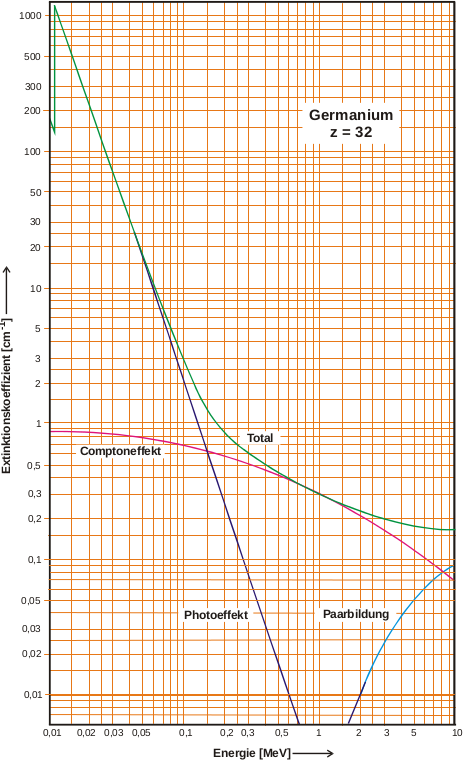
\includegraphics[scale=0.7]{/home/martin/Dokumente/SS14/Praktikum/V704/theorie.png}
\caption{Energieabhängigkeit des Absorptionskoeffizienten $\mu$ für Germanium getrennt nach den verschiedenen Wechselwirkungsmechanismen sowie Totaleffekt [1]}
\label{a1}
\end{figure}
So ist bei den niedrigen Energien der Fotoeffekt dominierend, schon bei mittleren Energien kann er hingegen vernachlässigt werden. Der Compton-Effekt ist bei geringen Energien zwar vorhanden, spielt aber erst bei mittleren Energien eine Rolle. Die Paarbildung setzt erst bei \SI{1}{MeV} ein, ist aber zunächst vernachlässigbar. Bei \SI{100}{MeV}findet fast nur noch die Paarbildung statt.
\subsection{$\beta$-Strahlung}
\subsubsection{Entstehung und Eigenschaften der $\beta$-Strahlung}
$\beta$-Strahlung besteht aus positiven oder negativen Elektronen mit hoher kinetischer Energie. Diese Elektronen werden von Atomkernen mit einer instabilen Anzahl von Protonen oder Neutronen emittiert. Zusätzlich zu dem Elektron wird ein Antineutrino $\overline{\nu}_e$ bzw. das Neutrino $\nu_e$ emittiert. Da die Energie, die bei der Kernumwandlung frei wird, statistisch auf das Elektron, das Neutrino und auf den Rückstoßkern verteilt wird, ist das Spektrum eines $\beta$-Strahlers kontinuierlich. Die bei der Kernwandlung freigewordene Energie entspricht dabei der Maximalenergie $E_{max}$ des Elektrons. Durch das emittierte (Anti-)Neutrino wird die Einhaltung aller Erhaltungssätze gewährleistet.
\subsubsection{Wechselwirkung von $\beta$-Strahlung mit Materie}
Aufgrund ihrer Ladung und ihrer im Vergleich zu anderen Teilchen geringen Masse ist ein $\beta$-Teilchen für sehr viele Wechselwirkungen verantwortlich. Es treten vor allem drei Prozesse auf, die im Folgenden näher erläutert werden.
\paragraph{Elastische Streuung am Atomkern}
Bei dieser sogenannten Rutherford-Streuung werden die $\beta$-Teilchen im Coulombfeld der Atomkerne zum Teil mit großem Winkel abgelenkt. Durch diese Auffächerung der Teilchen wird die Intensität verringert. Darüber werden die Bahnlängen durch die Absorberschicht erheblich größer als die Reichweite der Elektronen. Dieser Effekt ist in Abbildung \ref{a2} dargestellt. 
\begin{figure}[h]
\centering
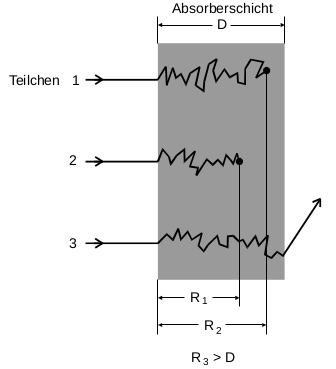
\includegraphics[scale=0.6]{abb2.png}
\caption{Veranschaulichung des Unterschiedes zwischen Bahnlänge und Reichweite individueller $\beta$-Teilchen in einer Materieschicht[1]}
\label{a2}
\end{figure}
Da die elastische Streuung unter relativistischen Geschwindigkeiten stattfindet, müssen die Rutherfordschen Streuformeln mehrfach korrigiert werden. Darauf soll hier aber nicht weiter eingegangen werden.
\paragraph{Inelastische Streuung am Atomkern}
Bei der inelastischen Streuung wird Energie in Form von Bremsstrahlung abgegeben, da die Elektronen im Coulombfeld eines Kerns beschleunigt werden. Die Wahrscheinlichkeit dieses Prozesses wird bestimmt durch den Wirkungsquerschnitt $\sigma{Br}$. Bezogen auf den Atomkern ergibt sich
\begin{equation}
\sigma_{Br} = \alpha r_e^2 z^2.
\label{8}
\end{equation}
Folglich spielt die Bremsstrahlung nur bei schweren Atomkernen eine Rolle. Die mittlere in Bremsstrahlung umgewandelte Energie eines $\beta$-Teilchens bei Durchgang durch die Materieschicht beträgt
\begin{equation}
E_{Br}[keV] \approx 7*10^{-7}zE_{\beta}^2
\label{9}
\end{equation}
Allerdings ist diese Formel nur für Energien bis ca. 2500 keV gültig. Insgesamt hat die Bremsstrahlung nur einen kleinen Anteil an den Energieverlusten der $\beta$-Teilchen.
\paragraph{Inelastische Streuung an Elektronen des Absorbermaterials}
Bei der Absorption von $\beta$-Strahlung müssen Energieverluste bis zur Energie Null erklärt werden. Die daher notwendige dritte Art der Wechselwirkung ist die Inelastische Streuung an Elektronen. Durch diese Streuung werden die Kerne ionisiert und angeregt. Durch die nur geringe Umwandlung von Energie kann ein Elektron viele dieser Wechselwirkungen durchlaufen. Die Wahrscheinlichkeit dieser inelastischen Streuung ist proportional zur Anzahl der Elektronen pro Volumeneinheit. Bei Aluminium und einer Elektronenenergie von 100 keV werden $\beta$-Teilchen schon bei einer Schichtdicke des Aluminiums von ca. 0.15 mm vollständig abgebremst.
\subsubsection{Die Absorptionskurve von $\beta$-Strahlung}
Aufgrund der Komplexität der Absorptionsvorgänge bei $\beta$-Strahlung ist die Aufstellung des Zusammenhangs zwischen der Intensität der Strahlung und der Dicke des Absorbers ein hier nicht lösbares Problem. Allerdings zeigt sich, dass für kleine Schichtdicken und natürliche Strahler mit guter Näherung das Apsorptionsgesetz in Formel (\ref{3}) gilt. Ist die Schichtdicke allerdings zu nahe an der maximalen Reichweiter der Elektronen, kann dieses Gesetz nicht angewendet werden. Abbildung \ref{a3} zeigt eine typische Absorptionskurve.
\begin{figure}[h]
\centering
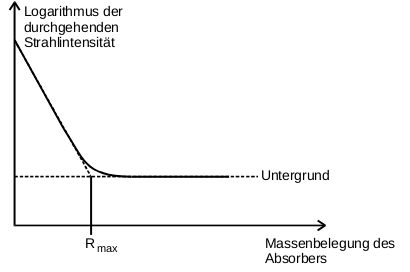
\includegraphics[scale=0.9]{abb3.png}
\caption{Absorptionskurve für einen natürlichen $\beta$-Strahler[1]}
\label{a3}
\end{figure}
 Die mit "Untergrund" bezeichnete Strahlenintensität setzt sich aus der Hintergrundstrahlung und der emittierten Bremsstrahlung der Elektronen zusammen. Um an der Absorptionskurve die maximale Reichweite der Elektronen zu bestimmen, verlängert man die beiden geraden Stücke des Graphen und liest die Reichweite im Schnittpunkt ab. Aus dieser Reichweite $R_{max}$ kann man die kernphysikalisch interessante Größe $E_{max}$ ermitteln. Aufgrund der so komplizierten Wechselwirkung ist der Zusammenhang aber nur empirisch. In unserem Experiment gilt
\begin{equation}
E_{max} = 1.92\sqrt{R_{max}^2 + 0.22 R_{max}}\, [MeV].
\label{10}
\end{equation}
\section{Vorbereitung und Durchführung}
\subsection{Aufbau}
Der grundlegende Versuchsaufbau ist der Abbildung \ref{a4} zu entnehmen. 
\begin{figure}[htp]
\centering
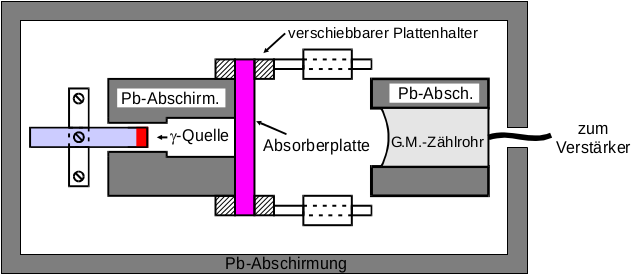
\includegraphics[scale=0.7]{abb4.png}
\caption{Schematische Darstellung der Messapparatur für die $\gamma$-Absorption[1]}
\label{a4}
\end{figure}
Ein Geiger-Müller-Zählrohr ist verstärkt an einem Zählwerk angeschlossen, die Messzeit ist einstellbar. Zwischen der strahlenden Probe und dem Zählrohr können Absorptionskörper in verschiedenen Stärken befestigt werden. Die Versuchsumgebung ist mit einer Bleiwand abgeschirmt.
\subsection{Durchführung}
Bevor die Probe eingesetzt wird, wird zunächst die Hintergrundstrahlung gemessen. Um eine hohe Genauigkeit zu erreichen, wird der Nulleffekt 900 Sekunden lang gemessen. In der folgenden Messung mit der Probe wird die Schichtdicke des Absorbers Schritt für Schritt erhöht, bei der Messung der $\beta$-Strahlung so lange, bis die Zählrate in der statistischen Schwankung konstant bleibt.\newline
Um eine geringere Strahlenbelastung zu erreichen, misst jede Praktikumsgruppe nur eine Strahlenart. Hier wird die $\beta$-Strahlung gemessen. Die Messwerte zur $\gamma$-Strahlung werden von unserer Partnergruppe bereitgestellt.
\section{Auswertung}
\subsection{Bestimmung der Messungenauigkeiten der Zählraten}
Da es sich beim radioaktiven Zerfall um einen statistischen Prozess handelt, soll hier die Berechnung der Messunsicherheiten noch einmal behandelt. Der Zerfall der Kerne lässt sich durch eine Poisson-Verteilung beschreiben. Daher beträgt der statistische Fehler der gemessenen Werte
\begin{equation}
\Delta N = \sqrt{N}.
\end{equation} 
Weil sich die Messapparatur nicht komplett abschirmen lässt, ist der sogenannte Nulleffekt zu berücksichtigen. Das ist die Anzahl der durch Hintergrundstrahlung ausgelösten Zählungen im Geiger-Müller-Zählrohr. Damit ergibt sich für den Fehler der Nettoaktivität $A-A_0$:
\begin{equation}
\Delta A = \sqrt{\left(\frac1{\Delta t}\right)^2 \cdot |N| +\left(\frac1{\Delta t_0}\right)^2 \cdot |N_0| }
\end{equation} 
Diese Größe wird im Folgenden in den Tabellen und in den Diagrammen (mittels Fehlerbalken) als Messunsicherheit der angegeben Aktivitäten angegeben. 
\paragraph{Anmerkung} Die Berechnung dieser Fehler, sowie die Erstellung der Diagramme und die lineare Ausgleichsrechnung wurden mit \textsc{Python} durchgeführt.  
\subsection{Bestimmung des Absorptionskoeffizienten $\mu$ von $\gamma$-Strahlung}
Die Absorptionskurven wurden jeweils für eine Schicht aus Kupfer und einer Schicht aus Blei aufgenommen. Die Tabellen 1 und 2 enthalten die über einen Zeitraum von 
\[
\Delta t_{Cu} = \SI{300}{\second}
\]
für Kupfer und
\[
\Delta t_{Pb} = \SI{100}{\second}
\]
für das Blei-Target gemessenen Werte und die entsprechenden Zählraten
\[
A = \frac{N}{\Delta t} - A_0.
\]
In den Abbildungen \ref{abb_gamma1_lin} und \ref{abb_gamma2_lin} sind die Absorptionskurven für die jeweiligen Metalle linear aufgetragen. 
\begin{figure}[H]
\centering
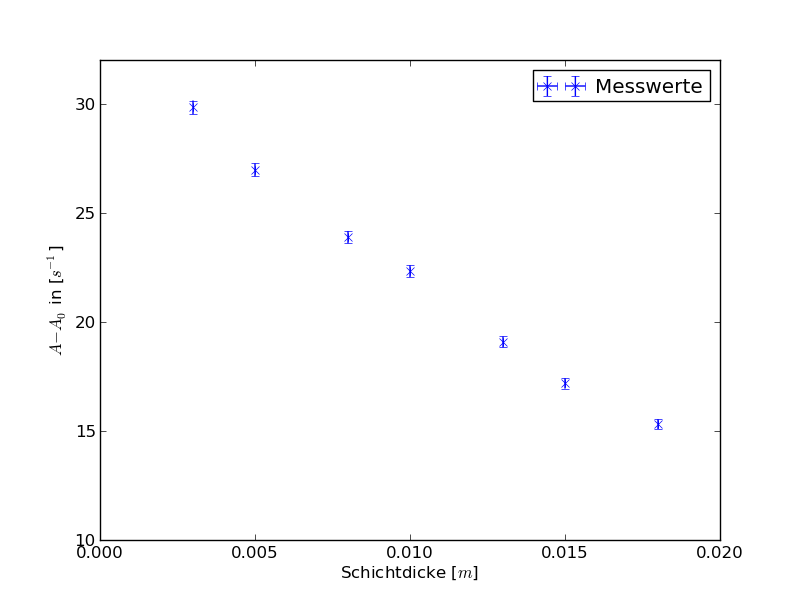
\includegraphics[scale=0.6]{/home/martin/Dokumente/SS14/Praktikum/V704/gamma1_lin.png}
\caption{Linearer Plot der gemessenen Aktivität in Abhängigkeit von der Schichtdicke $d$ für das Cu-Target}
\label{abb_gamma1_lin}
\end{figure}
\begin{figure}[H]
\centering
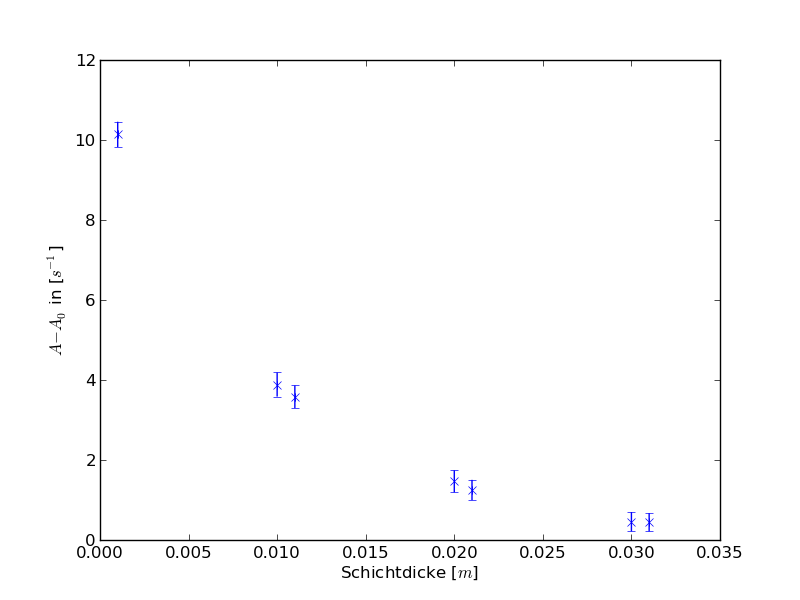
\includegraphics[scale=0.6]{/home/martin/Dokumente/SS14/Praktikum/V704/gamma2_lin.png}
\caption{Linearer Plot der gemessenen Aktivität in Abhängigkeit von der Schichtdicke $d$ für das Pb-Target}
\label{abb_gamma2_lin}
\end{figure}

\begin{figure}[H]
\centering
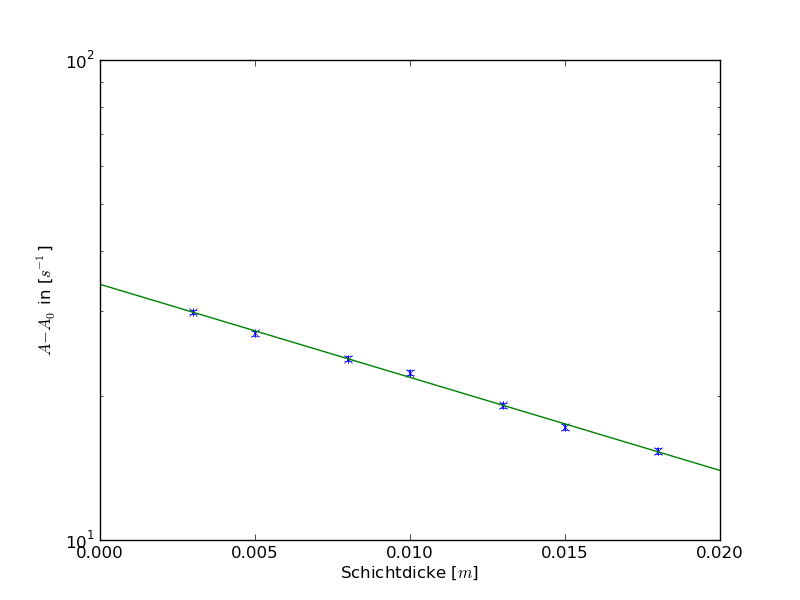
\includegraphics[scale=0.6]{/home/martin/Dokumente/SS14/Praktikum/V704/gamma1_log.png}
\caption{Halblogarithmischer Plot der gemessenen Aktivität in Abhängigkeit von der Schichtdicke $d$ für das Cu-Target}
\label{abb_gamma1_log}
\end{figure}
\begin{figure}[H]
\centering
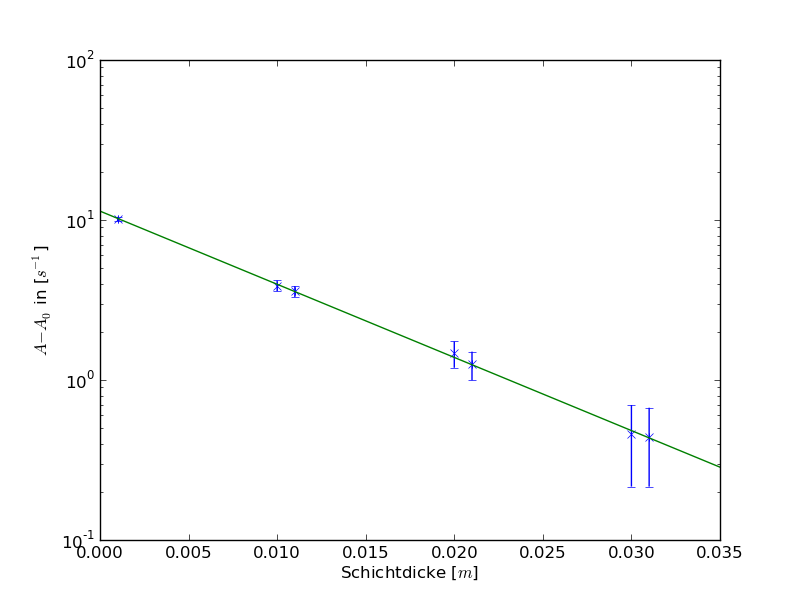
\includegraphics[scale=0.6]{/home/martin/Dokumente/SS14/Praktikum/V704/gamma2_log.png}
\caption{Halb-logarithmischer Plot der gemessenen Aktivität in Abhängigkeit von der Schichtdicke $d$ für das Pb-Target}
\label{abb_gamma2_log}
\end{figure}
\noindent
Zur Berechnung der Absorptionskoeffizienten wurden diese Werte auch halb-logarithmisch aufgetragen (Abbildungen \ref{abb_gamma1_log}  und \ref{abb_gamma2_log}) und eine lineare Ausgleichsrechnung 
\[
\ln{A} = \mu \cdot d + \ln{A(0)}
\]
durchgeführt. Die folgenden Werte wurden bestimmt:
\begin{table}[h]
\centering
\begin{tabular}{lll}

\toprule
	Material & $\frac{\mu}{\si{\meter^{-1}}} $& $\ln{A(0)}$ \\
 \midrule 
 	Cu & \num{44.6+-0.9} & \num{3.529+-0.011}\\
	Pb & \num{-05.3+-1.3}  & \num{2.430+-0.027}\\

\bottomrule
\end{tabular}
\end{table}

\noindent
Hieraus lässt sich durch Anwendung der Exponentialfunktion die Zählrate des Strahlers ohne Abschirmung $A(0)$ berechnen:
\begin{itemize}
\item $A_{Cu}(0)$ = \SI{34.1+-0.4}{\becquerel}
\item $A_{Pb}(0)$ = \SI{11.4+-0.3 }{\becquerel}.

\end{itemize}
\paragraph{Theoretische Berechnung von $\mu$}
Zur Berechnung des Wirkungsquerschnitts $\sigma_{com}$ muss zunächst das Verhältnis von Quantenenergie zur Ruheenergie des Elektrons berechnet werden. Der Verwendete Strahler ${}^{137}$Cs  hat eine Quantenenergie von $E_\gamma = \SI{0.662}{\kilo\eV}$[2]. Somit ergibt sich für 
\[
\epsilon =  \frac{E_\gamma}{m_ec^2} = \num{1.3}.
\]
Aus Formel \ref{6} berechnet $\sigma_{com}$ zu
\[
\sigma_{com} = \SI{2.76e-29}{\meter\squared}
\]
Aus diesem Wert kann aus Formel (\ref{7}). Dazu werden noch die Molare Masse $M$ sowie die Dichte $\rho$ des verwendeten Targets. Die folgende Tabelle zeigt die berechneten Werte:
\begin{table}[h]
\centering
\begin{tabular}{lllll}
\toprule
	Material & $Z$ & $\frac{M}{\si{\gram\per\mole}}$ &$\frac{\rho}{\si{\kilo\gram\per\meter\squared}}$ &$\frac{\mu}{\si{\meter^{-1}}}$ \\
\midrule
	Cu & 29 &63.546  &8.83 & 0.068\\
	Pb &82 & 207.2& 11.342 & 0.075    \\
\bottomrule
\end{tabular}
\label{tab_gamma2}
\end{table} 
\subsection{Bestimmung der $R_{Max}$ und der maximalen Energie der $\beta$-Strahlung}
Zur Bestimmung der Absorptionskurve von $\beta$-Strahlung wurde über einen Zeitraum von
\[
\Delta t = \SI{60}{\second}
\]
gemessen. Die Ergebnisse, sowie die daraus berechnete Zählrate
\[
A = \frac{N}{\Delta t}
\]
befinden sich in Tabelle \ref{tab_beta}. In Abbildung \ref{abb_beta} werden diese Daten halb-logarithmisch aufgetragen. Es zeigt sich der zu erwartende Kurvenverlauf. 
\begin{figure}[htp]
\centering
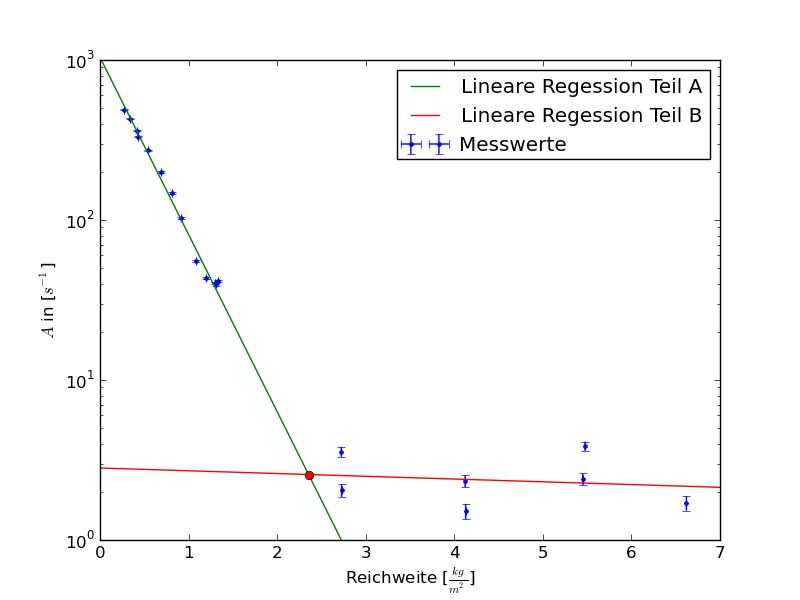
\includegraphics[scale=0.85]{/home/martin/Dokumente/SS14/Praktikum/V704/beta_log.png}
\caption{}
\label{abb_beta}
\end{figure}
\newpage
Eine lineare Ausgleichsrechnung
\[
\ln{A} = m\cdot d + b
\]
wird jeweils für die ersten 13 Messpunkte sowie für die restlichen Daten ausgeführt. Daraus ergeben sich folgende Werte:
\begin{table}[h]
\centering
\begin{tabular}{cSS}
	\toprule
	Gruppe & $m$ & $b$\\
	\midrule
	A & -6.88+-0.19e+3 & 6.95+-0.06 \\
	B & -1.1+-2.6e+02 & 1.0+-0.4\\
	\bottomrule
\end{tabular}

\end{table}
Die X-Koordinate des Schnittpunktes der beiden Ausgleichsgeraden entspricht der maximalen Einringtiefe $R_{Max}$. Hiermit ergibt sich:
\begin{equation}
R_{Max} = \frac{b_2-b_1}{m_1-m_2} = \SI{0.87+-0.08}{\milli\meter}.
\end{equation}

Aus diesem Wert kann mit Hilfe der empirischen Formel (\ref{10}) bestimmt werden.
\[
E_{Max} = 1.92\sqrt{R_{Max}^2+0.22R_{Max}}[\si{\mega\eV}] = \SI{0.0266+-0.0012}{\mega\eV}
\]
Der Theoriewert[3] für die Maximalenergie des hier verwendeten Strahlers ${}^{99}$Tc beträgt
\[
E_{Max} = \SI{0.314+-0.018}{\mega\eV}.
\]
Damit beträgt die relative Abweichung des experimentell ermittelten Werts:
\[
\Delta E_{max} = \SI{-6.8}{\percent}
\]
\section{Diskussion}

Die im ersten Versuchsteil aufgenommen Daten bestätigen die theoretischen Überlegungen zur $\gamma$-Absorption. Die erwartete exponentielle Abhängigkeit von der Schichtdicke $d$ konnte sowohl für Kupfer, als auch für Blei nachgewiesen werden. Dennoch stimmen ermittelten Werte für $\mu$ nicht mit den berechneten Zahlen für den Compton-Absorptionskoeffizienten $\mu_{com}$ überein. Hieraus kann geschlossen werden, dass der Compton-Effekt bei der Absorption von $\gamma$-Strahlung in dem hier Untersuchten Energiebereich eine untergeordnete Rolle spielt. Problematisch sind auch die unterschiedlichen Werte für die Aktivität ohne Target $A(0)$. Diese sollten theoretisch gleich sein, da es bei einer Schichtdicke von $d = \SI{0}{\milli\meter}$ keine Materialabhängigkeit der Aktivität geben dürfte.

\noindent
Die Ergebnis der Untersuchung mit $\beta$-Strahlung an Aluminium ist mit einer relativen Abweichung von \SI{-6.8}{\percent} mit dem Theoriewert verträglich.

\noindent
\newpage
\section{Quellen}
\begin{enumerate}[{[}1{]}]
\item Entnommen der Praktikumsanleitung \textit{Absorption von $\gamma$- und $\beta$-Strahlung} der TU Dortmund. Download am 21.04.14 unter:\\
 \url{http://129.217.224.2/HOMEPAGE/PHYSIKER/BACHELOR/AP/SKRIPT/V351.pdf}
 \item Entommen aus: \textit{RADIONUCLIDE SAFETY DATA SHEET}, Stanford University.\\ Download am 21.04.14 unter:\\
\url{http://www.stanford.edu/dept/EHS/prod/researchlab/radlaser/RSDS_sheets/Cs-137.pdf}
 \item Kaplan, Irving, \textit{Nuclear Physics}, New York: Addison-Wesley, 1964.
\end{enumerate}
\section{Anhang}
\begin{itemize}
\item Tabellen
\item Auszug aus dem Messheft
\end{itemize}
\newpage

\begin{table}
\centering
\begin{tabular}{ScS}
\toprule
{{$\frac{d}{\si{\milli\meter}}$} } &{ $N$} &{ { $\frac{A-A_0}{\si{\second^{-1}}}$ } }\\
\midrule
3 & 9003 & 29.83+-0.32\\
5 & 8144 & 26.96+-0.30\\
8 & 7219 & 23.88+-0.28\\
10 & 6751 & 22.32+-0.27\\
13 & 5779 & 19.08+-0.25\\
15 & 5209 & 17.18+-0.24\\
18 & 4649 & 15.31+-0.23\\
\bottomrule
\end{tabular}
\label{tab_gamma1}
\caption{Ergebnisse der Messung des $\gamma$-Strahlers an einem Cu-Target.}
\end{table}



\begin{table}
\centering
\begin{tabular}{SSS}
\toprule
{{$\frac{d}{\si{\milli\meter}}$} } &{ $N$} &{ { $\frac{A-A_0}{\si{\second^{-1}}}$ } }\\
\midrule
1 & 3097 & 10.14+-0.32\\
10 & 1221 & 3.89+-0.30\\
11 & 1129 & 3.58+-0.28\\
20 & 495 & 1.47+-0.27\\
21 & 430 & 1.25+-0.25\\
30 & 192 & 0.46+-0.24\\
31 & 188 & 0.44+-0.23\\
\bottomrule
\end{tabular}
\label{tab_gamma2}
\caption{Ergebnisse der Messung des $\gamma$-Strahlers an einem Pb-Target.}
\end{table}



\begin{table}
\centering
\begin{tabular}{SSS}
\toprule
{$\frac{d}{\si{\micro\meter}}$} &{ $N$} &{ $\frac{A}{\si{\second^{-1}}}$ }\\
\midrule
102 & 2.942+-0.017e+04 & 490.4+-2.9\\
126 & 2.578+-0.016e+04 & 429.7+-2.7\\
153 & 2.163+-0.015e+04 & 360.5+-2.5\\
160 & 1.984+-0.014e+04 & 330.6+-2.3\\
199 & 1.642+-0.013e+04 & 273.6+-2.1\\
252 & 1.197+-0.011e+04 & 199.4+-1.8\\
301 & 8.83+-0.09e+03 & 147.2+-1.6\\
338 & 6.19+-0.08e+03 & 103.1+-1.3\\
399 & 3.34+-0.06e+03 & 55.6+-1.0\\
444 & 2.60+-0.05e+03 & 43.4+-0.9\\
481 & 2.42+-0.05e+03 & 40.4+-0.8\\
483 & 2.38+-0.05e+03 & 39.6+-0.8\\
491 & 2.50+-0.05e+03 & 41.6+-0.8\\
\midrule
1008 & 214.0+-14.6 & 3.57+-0.25\\
1010 & 123.0+-11.1 & 2.05+-0.19\\
1527 & 140.0+-11.8 & 2.33+-0.20\\
1529 & 91.0+-10.0 & 1.52+-0.16\\
2019 & 144.0+-12.0 & 2.40+-0.20\\
2027 & 232.0+-15.2 & 3.87+-0.26\\
2451 & 102.0+-10.1 & 1.70+-0.17\\
\bottomrule
\end{tabular}
\label{tab_beta}
\caption{Ergebnisse der Messung des $\beta$-Strahlers an einem Al-Target.}
\end{table}



\end{document}